\documentclass[
  captions=tableheading,
  bibliography=totoc, 
  titepage=firstiscover,
]{scrartcl}

\usepackage{blindtext} %neuer input

\usepackage{longtable} % Tabellen über mehrere Seiten

\usepackage[utf8]{inputenc} %neuer input

\usepackage{scrhack}

\usepackage[aux]{rerunfilecheck} %Warnung falls nochmal kompiliert werden muss

\usepackage{fontspec} %Fonteinstellungen

\recalctypearea{}

\usepackage[main=ngerman]{babel} %deutsche Spracheinstellung

\usepackage{ragged2e} %neuer input

\usepackage{amsmath, nccmath}

\usepackage{amssymb} %viele mathe Symbole

\usepackage{mathtools} %Erweiterungen für amsmath


\DeclarePairedDelimiter{\abs}{\lvert}{\rvert}
\DeclarePairedDelimiter{\norm}{\lVert}{\rVert}

\DeclarePairedDelimiter{\bra}{\langle}{\rvert}
\DeclarePairedDelimiter{\ket}{\lvert}{\rangle}

\DeclarePairedDelimiterX{\braket}[2]{\langle}{\rangle}{
#1 \delimsize| #2
}

\NewDocumentCommand \dif {m}
{
\mathinner{\symup{d} #1}
}


\usepackage[
  math-style=ISO,
  bold-style=ISO,
  sans-style=italic,
  nabla=upright,
  partial=upright,
  warnings-off={
    mathtools-colon,
    mathtools-overbracket,
  },
]{unicode-math}

\setmathfont{Latin Modern Math}
\setmathfont{XITS Math}[range={scr, bfscr}]
\setmathfont{XITS Math}[range={cal, bfcal}, StylisticSet=1]


\usepackage[
  locale=DE,
  separate-uncertainty=true,
  per-mode=reciprocal,
  output-decimal-marker={,},
]{siunitx}

\usepackage[autostyle]{csquotes} %richtige Anführungszeichen

\usepackage{xfrac}

\usepackage{float}

\floatplacement{figure}{htbp}

\floatplacement{table}{htbp}

\usepackage[ %floats innerhalb einer section halten
  section,   %floats innerhalb er section halten
  below,     %unterhalb der Section aber auf der selben Seite ist ok
]{placeins}

\usepackage[
  labelfont=bf,
  font=small,
  width=0.9\textwidth,
]{caption}

\usepackage{subcaption} %subfigure, subtable, subref

\usepackage{graphicx}

\usepackage{grffile}

\usepackage{booktabs}

\usepackage{microtype} %Verbesserungen am Schriftbild

\usepackage[
backend=biber,
]{biblatex}

\addbibresource{../lit.bib}

\usepackage[ %Hyperlinks im Dokument
  german,
  unicode,
  pdfusetitle,
  pdfcreator={},
  pdfproducer={},
]{hyperref}

\usepackage{bookmark}

\usepackage[shortcuts]{extdash}

%\usepackage{warpcol}


\begin{document}
    \title{V603 Compton-Effekt}
    \author{  
    Tobias Rücker\\
    \texorpdfstring{\href{mailto:tobias.ruecker@tu-dortmund.de}{tobias.ruecker@tu-dortmund.de}}{}}
    
    \date{ Abgabe: 05.05.2020 \vspace{-4ex}}
\maketitle
\thispagestyle{empty}

\newpage
\tableofcontents
\thispagestyle{empty}
\newpage

% Ziel %%%%%%%%%%%%%%%%%%%%%%%%%%%%%%%%%%%%%%%%%%%%%%%%%%%%%%%%%%%%%%%%%%%%%%%%%%%%%%%%%%%%%%%%%%%%%%%%%%%%%%%%%%%%%%%%%%%%%%%%%%%%%%%%%%%%%%%%%%%%%%%%%%%%%%%%%%%%%%%%%%%%%%%%%%%%%%%%%%%%%%%%%%%%%%%%%%%%%%%%%%%%%%%%%

\setcounter{page}{1}
\section{Ziel}\justifying

Der Compton-Effekt stellt in der Physik eine gute Methode dar, um zum Beispiel die Richtung der Herkunft hochenergetischer 
Strahlung zu bestimmen oder um Atome mittels Laser-Kühlung auf tiefe Temperaturen zu bringen. 
Daher wird in einem Experiment die Comptonwellenlänge, zum näheren Verständnis des Compton-Effekts,
mittels der Transmission eines Aluminium-Absorbers bestimmt werden.

% Theorie %%%%%%%%%%%%%%%%%%%%%%%%%%%%%%%%%%%%%%%%%%%%%%%%%%%%%%%%%%%%%%%%%%%%%%%%%%%%%%%%%%%%%%%%%%%%%%%%%%%%%%%%%%%%%%%%%%%%%%%%%%%%%%%%%%%%%%%%%%%%%%%%%%%%%%%%%%%%%%%%%%%%%%%%%%%%%%%%%%%%%%%%%%%%%%%%%%

\section{Theorie}\justifying

Bei der Bestrahlung von Kristallen mit Röntgenlicht wird beobachtet, dass
bei verschiedenen Winkeln Wellenlängen nicht nur die Wellenlänge des eingestrahlten Lichts gefunden wird,
sondern auch eine Wellenlänge, die größer als die eingestrahlte Wellenlänge ist.\\
Dieses Phänomen ist auf den Compton-Effekt zurückzuführen. Dieser beschreibt,
dass ein einfallendes Photon einen Teil seiner Energie an ein freies Elektron abgibt
und in einem Winkel $\theta $ zur einfallenden Strahlung gestreut wird. Die Energie des Photons wird 
dabei beschrieben durch die Gleichung 
\begin{align}
    E  = \hbar \omega \label{eq:1}.
\end{align}
Dabei bezeichnet $\hbar $ das verschränkte plancksche Wirkungsquantum und $\omega $
Aus Energie- und Impulserhaltung lässt sich die Differenz der beiden Wellenlängen bestimmen \cite{V603}
\begin{align}
    \Delta \lambda = \lambda _2 - \lambda _1 = \frac{h}{m_e c}(1-\cos(\theta))  \label{eq:2},
\end{align}
wobei $\lambda _2 $ die Wellenlänge der Compton-Streuung, $\lambda _1 $ die Wellenlänge
der einfallenden Strahlung und $\theta$ den Streuwinkel der Strahlung definiert. Die Konstante $\frac{h}{m_e c}$ wird als
Compton-Wellenlänge bezeichnet und hat dementsprechend die Dimension einer Länge,
wobei $m_e$ die Masse des Elektrons, h das planksche Wirkungsquantum und c die Lichtgeschwindigkeit im
Vakuum ist.\\
Um Röntgenstrahlung für eine Messung zu erzeugen werden Elektronen aus einer 
Glühkathode  auf eine Anode beschleunigt. Das Spektrum der Emission
setzt sich dann aus zwei Bestandteilen zusammen, der Bremsstrahlung und
der charakeristischen Röntgenstrahlung.
Die Bremsstrahlung entsteht durch den Energieverlust bei der Abbremsung durch
das E-Feld eines Atoms. Das ausgestrahlte Photon besitzt dann genau den
durch die Abbremsung verlorene Energie, wodurch das Spektrum der Bremsstrahlung kontinuierlich
ist. 
Die charakteristische Strahlung entsteht, indem ein Elektron ein Atom ionisiert.
Dadurch fällt ein Elektron von einer äußeren Schale unter Emission eines 
Röntgenquants ins Innere. Die charakteristische Strahlung hängt
dabei vom Anodenmaterial ab und durch die quantisierten Energiezustände von Atomen
sind diese Linien scharf.\\
Durch Transmission und Absorption von Röntgenstrahlung durch Aluminium kann
die Compton-Wellenlänge ermittelt werden. Die Transmission durch verschiedene Stoffe
verringert sich mit steigender Wellenlänge, wodurch die Intensität
Compton-Wellenlänge geringer wird. Berechnen lässt sich der Transmissionskoeffizient durch
\begin{align}
    T=\frac{I}{I_0} \label{eq:3}.
\end{align}
$I_0$ beschreibt hierbei die Intensität der gesamten einfallenden Strahlung und I
die transmittierte Strahlung, die gerde betrachtet wird.
\flushleft{Die\,}\justifying Absorption verringert wiederum 
 die Intensität der einfallenden Strahlung.\\
Die Wellenlänge $\lambda$ kann hierbei durch die Bragg'sche Bedingung bestimmt 
werden
\begin{align}
    2d \sin (\alpha)=n \lambda \label{eq:4}.
\end{align}
$\lambda$ ist dabei die im Winkel $\alpha$ gebeugte Wellenlänge, d die Gitterkonstante und n die Interferenzordnung.


% Versuchsaufbau + Versuchsdurchführung %%%%%%%%%%%%%%%%%%%%%%%%%%%%%%%%%%%%%%%%%%%%%%%%%%%%%%%%%%%%%%%%%%%%%%%%%%%%%%%%%%%%%%%%%%%%%%%%%%%%%%%%%%%%%%%%%%%%%%%%%%%%%%%%%%%%%%%%%%%%%%%%%%%%%%%%%%%%%%%%%%%%%%%%%%%%%%%%%%%%%%%%%%%%%%%%%%

\section{Versuchsaufbau und Versuchsdurchführung}\justifying

Zuerst wird der Aufbau für die Bestimmung des Emissionsspektrums von Kupfer aufgebaut.
Dafür wird das Röntgengerät 
\begin{figure}[H]
    \centering
    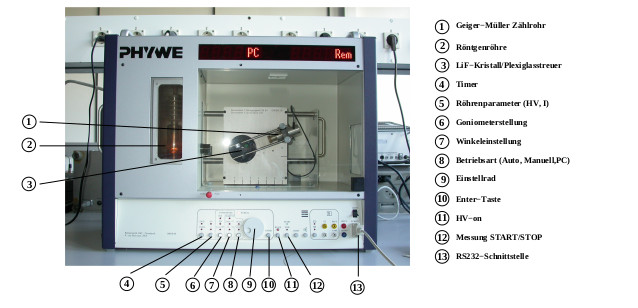
\includegraphics[width=\linewidth]{./images/Aufbau1.jpg}
    \caption{Aufbau einer Röntgenröhre \cite{V603}}
    \label{fig:1}
\end{figure}
\flushleft{mit\,} \justifying dem PC über RS232-Kabel verbunden und ein  LiF-Kristall sowie eine 2 mm Blende in die Röntgenröhre eingebracht. Dann wird mihilfe
eines Computerprogramms eine Integrationszeit zwischen 5-10s eingestellt, die Schrittweite auf 0,1°
festgelegt und der Winkelbereich gewählt so, dass der gesamte Bremsberg sowie die
charakteristischen Linien enthalten sind. \\
Für die Aufnahme der Transmission des Aluminium-Absorbers wird dieser vor die 2mm Blende gesetzt
und eine Messung mit dem Absorber sowie eine ohne den Absorber durchgeführt bei einer Messzeit von 100s.
\flushleft{Für\,}\justifying die Messung der Comptonwellenlänge wird zuerst die Intensität der Kupferröhre gemessen.
Dafür wird nun eine 5mm Blende statt der 2mm Blende verwendet und der LiF-Kristall
durch einen Plexiglasstreuer ausgetauscht. Das RS232-Kabel wird entfernt und es wird
eine manuelle Messung durchgeführt. Dafür wird der Kristall auf 45° und das Geiger-Müller Zählrohr auf 90°
eingestellt. Danach wird die Intensität der Cu-Röhre gemessen.\\
Zuletzt wird die Intensität mit Aluminium-Absorber in 2 verschiedenen Stellungen bei einer Messzeit von mindestens 300s
gemessen: 
\begin{figure}[H]
    \centering
    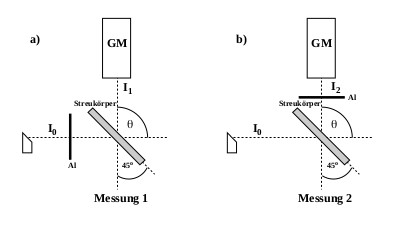
\includegraphics[width=\linewidth]{./images/Aufbau2.jpg}
    \caption{Aufbau der 2  Stellungen im Röntgengerät zur Messung der Intensität \cite{V603}}
    \label{fig:2}
\end{figure}
\flushleft{Diese\,}\justifying Messung in den 2 Stellungen wird 5 mal wiederholt.

% Auswertung %%%%%%%%%%%%%%%%%%%%%%%%%%%%%%%%%%%%%%%%%%%%%%%%%%%%%%%%%%%%%%%%%%%%%%%%%%%%%%%%%%%%%%%%%%%%%%%%%%%%%%%%%%%%%%%%%%%%%%%%%%%%%%%%%%%%%%%%%%%%%%%%%%%%%%%%%%%%%%%%%%%%%%%%%%%%%%%%%%%%%%%%%%%%%%%%%%

\section{Auswertung}

Für alle Messungen ist eine Spannung von \SI{35}{\kilo\volt} und ein
Emissionsstrom von \SI{1}{\milli\ampere} verwendet worden.
Alle Graphiken in der Auswertung sind mit dem Programm
Matplotlib \cite{matplotlib} erstellt worden.
Alle Messungenauigkeiten wurden mit Uncertainties \cite{uncertainties} berechnet.

\flushleft{Die\,} Gitterkonstante des LiF-Kristalls lautet \cite{V603}
\begin{align}
    d_{LiF}=\SI{201,4}{\pico\meter} \label{eq:5}.
\end{align}

\subsection{Emissionsspektrum Kupfer}

\flushleft{Die\,}\justifying Messwerte für das Emissionsspektrum von Kupfer sind in der nachfolgenden Tabelle 
aufgetragen.


\input{table_Cu.tex}




Die Graphik für die Messwerte aus der Tabelle \ref{tab:1} ergibt den Plot:
\begin{figure}[H]
    \centering
    \includegraphics[width=\linewidth]{./build/plot_Cu.pdf}
    \caption{Emissionsspektrum von Kupfer \cite{matplotlib}}
    \label{fig:3}
\end{figure}

\flushleft{Aus\,}\justifying der Graphik lassen sich die Werte für die $K_{\alpha}$- und$K_{\beta}$-Linie
ablesen. $K_{\alpha}$ liegt bei ca. 22,5°$\pm$ 0,1° und $K_{\beta}$ bei ca. 20,1°$\pm$ 0.1°.
Daraus lässt sich mit Gleichung \eqref{eq:4} für $n=1$ die Wellenlänge berechnen:
\begin{align}
    \lambda _{\alpha}&= \SI{1,54+-0,006e-10}{\meter} \label{eq:6}\\
    \lambda_{\beta}&= \SI{1,38+-0,007e-10}{\meter} \label{eq:7}
\end{align}
Damit kann die Energie mithilfe der Gleichung \eqref{eq:1} der Linien bestimmt werden:
\begin{subequations}
\begin{align}
    E_{\alpha}&= \hbar \omega _{\alpha} = \frac{h c}{\lambda _{\alpha}}=\SI{8043+-34}{\electronvolt}  \label{eq:8a} \\
    E_{\beta}&= \SI{8,96+-0.04e03}{\electronvolt} \label{eq:8b}
\end{align}
\end{subequations}

\flushleft{Für\,}\justifying die Konstanten h und c werden die Werte von dem Programm Scipy  \cite{scipy} verwendet.

\subsection{Transmission bei Aluminium}

Die Messwerte für das $\lambda T$-Diagramm lauten:  

\begin{table}[H]
    \centering
    \input{table_Al.tex}
    \caption{Messwerte für das Transmissionsspektrum von Aluminium}
    \label{tab:2}
\end{table}


\flushleft{Für\,}\justifying den Graphen werden die Wellenlängen mit den Winkeln aus Tabelle \ref{tab:2}
mit Gleichung \eqref{eq:4} und $n=1$ berechnet.
Für die Berechnung Transmissionwerte wird Gleichung \eqref{eq:3} verwendet.
Für die Bestimmung der Intensität muss noch eine Totzeitkorrektur mit einer
Totzeit von $\tau = \SI{60}{\micro\second} $ durchgeführt werden:
\begin{align}
    I = \frac{N}{1-\tau \cdot N} \label{eq:9}.
\end{align}

\begin{figure}[H]
    \centering
    \includegraphics[width=\linewidth]{./build/plot_T.pdf}
    \caption{Transmission von Aluminium \cite{matplotlib}}
    \label{fig:4}
\end{figure}

\flushleft{Die} Fitparameter der Geraden 
\begin{equation}
    T=a \lambda +b \label{eq:10}
\end{equation}
sind mit SciPy \cite{scipy} berechnet worden und betragen 
\begin{align}
    a &= \text{\input{a_Al.tex}}\quad \text{und} \label{eq:11} \\
    b &= \text{\input{b_Al.tex}}.\label{eq:12}
\end{align}

Die drei gemessenen Intensitäten $I_0, I_1$ und $I_2$ für die Bestimmung der Comptonwellenlänge
haben die Werte
\begin{subequations}
\begin{align}
    I_0 &= 2731\pm 50 \,\text{Impulse} \label{eq:13a}, \\
    I_1 &= 1180 \pm 34\,\text{Impulse}\, \label{eq:13b} \text{und} \\
    I_2 &=1024\pm 32 \,\text{Impulse}\label{eq:13c}.
\end{align}
\end{subequations}

Damit wird die Transmission von Aluminium mit Gl. \eqref{eq:5} berechnet:
\begin{subequations}
\begin{align}
    T_1 &= 0,432\pm 0,015 \label{16a}\\
    T_2 &= 0,375\pm 0.014 \label{16b} 
\end{align}
\end{subequations}

Durch Umstellen der Gl. \eqref{eq:12} wird mit den Transmissionskoeffizienten
die Wellenlängen $\lambda _1$ und $\lambda _2$ berechnet
\begin{subequations}
\begin{align}
    \lambda &= \frac{T-b}{a} \label{17a}\\
    \lambda _1 &= \SI{52,2+-1.6}{\pico\meter} \label{17b}\\
    \lambda _2 &= \SI{55,9+-1.6}{\pico\meter} \label{17c}.
\end{align}
\end{subequations}

Daraus lässt sich die Comptonwellenlänge nach Formel \eqref{eq:2} mit $\theta = 90°$
bestimmen:
\begin{align}
    \lambda _c = \lambda _2 - \lambda _1 = \SI{3,8+-1,1}{\pico\meter} \label{eq:18}
\end{align}


% Diskussion %%%%%%%%%%%%%%%%%%%%%%%%%%%%%%%%%%%%%%%%%%%%%%%%%%%%%%%%%%%%%%%%%%%%%%%%%%%%%%%%%%%%%%%%%%%%%%%%%%%%%%%%%%%%%%%%%%%%%%%%%%%%%%%%%%%%%%%%%%%%%%%%%%%%%%%%%%%%%%%%%%%%%%%%%%%%%%%%%%%%%%%%%%%%%%%%%%

\section{Diskussion}

In der nachfolgenden Tabelle sind die für die Diskussion benötigten Werte, ihre Literaturwerte und
die dazugehörigen relativen Fehler zusammengefasst.
\begin{table}[H]
\centering
\begin{tabular}{c c c c}
\toprule
\multicolumn{2}{c}{Messwert}& \multicolumn{1}{c}{Literaturwert}& \multicolumn{1}{c}{relativer Fehler} \\
\cmidrule(lr){1-4} 
$K_{\alpha}$    &   \SI{8043+-34}{\electronvolt} & \SI{8048}{\electronvolt} \cite{K_Linie} & $6,21\cdot 10^{-2 }\%$\\
$K_{\beta} $    &   \SI{8,96+-0.04e03}{\electronvolt} & \SI{8905}{\electronvolt} \cite{K_Linie} & $0,61\%$\\
$\lambda _c $    &   \SI{3,8+-1,1}{\pico\meter} & \SI{2.43263}{\pico\meter} \cite{nolting2013grundlagen} & $54,97\%$\\
\bottomrule
\end{tabular}
\caption{gemessene Werte, Literaturwerte und relativer Fehler}
\label{tab:3}
\end{table}

\flushleft{Das\;}\justifying Kupferspektrum in Abbildung \ref{fig:3} gibt das zu erwartende Spektrum gut
wieder. Das Bremsspektrum ist kontinuierlich und die Intensität nimmt mit steigender Wellenlänge ab.
Neben dem Bremsspektrum sind klar die beiden Peaks zu erkennen, welche die $K_{\alpha} $-
und die $K_{\beta} $-Linie definieren. Im Vergleich zu den Literaturwerten in der Tabelle \ref{tab:3}
sind die Werte nah am gesuchten Wert, was sich in den geringen relativen Fehlern zeigt.
Auffällig an dem Graph ist, dass die $K_{\alpha} $-Linie wesentlich häufiger gemessen wurde
als die $K_{\beta}$-Linie. Das kommt vermutlich daher, dass $K_{\alpha} $ ein
geringeres Energieniveau besitzt als $K_{\beta} $ und dementsprechend die 
Elektronen häufiger diesen Schalenübergang ionisieren.\\
Für die Transmission des Aluminium-Absorbers zeigt die Abbildung
\ref{fig:4} einen linearen Zusammenhang zwischen Transmission und Wellenlänge,
was die geringen Messungenauigkeiten der Koeffizienten \eqref{eq:11} und \eqref{eq:12}
bestätigen.
Bei der Berechnung der Compton-Wellenlänge wird keine Totzeitkorrektur angewandt,
da durch die Totzeit von $\tau = \SI{60}{\micro\second} $ für kleine N in 
Gleichung \eqref{eq:9} der Nenner $\approx$ 1 ist und dann $I=N$ entspricht.
Die Comptonwellenlänge hat mit $54,97\%$ einen relativ großen Fehler. Dieser Fehler
kann zum Teil  durch Verunreinigungen im Plexiglasstreuer entstehen, wodurch auch andere 
Wellenlängen gemessen werden, die nicht mit gemessen werden sollten.
Zudem ist das Vakuum eventuell nicht perfekt, wodurch manche Elektronen mit
übrig gebliebenen Teilchen wechselwirken und Strahlung erzeugen. Zudem befindet sich im 
Bereich des Plexiglastreuer kein Vakuum, wodurch dort auch Teilchen in der Luft
ionisiert werden könnten. Außerdem wurde die Gerade in Abbildung \ref{fig:4} nur im
Bereich 7° bis 10° erstellt. Die Messung der Wellenlängen wurde allerdings
bei 45° gemacht, wo es möglich wäre, dass die Gerade für diesen Bereich nicht
die optimale Näherung darstelle. \\
Nichtsdestotrotz kann anhand der Comptonwellenlänge erkannt werden, warum spezifisch 
Röntgenstrahlung zur Untersuchung verwendet wurde. Die maximale Wellenlängenänderung
liegt bei 180° wodurch 
\begin{align}
    \Delta \lambda = 2 \cdot \lambda _c \approx \SI{5}{\pico\meter} \;\text{(nach dem Literaturwert)}
\end{align}
ist. Die maximale Wellenlängenänderung liegt im Bereich Picometer, wodurch sie zum Beispiel im sichtbaren Bereich von Nanometer
kaum einen Unterschied machen würde.



% Literatur %%%%%%%%%%%%%%%%%%%%%%%%%%%%%%%%%%%%%%%%%%%%%%%%%%%%%%%%%%%%%%%%%%%%%%%%%%%%%%%%%%%%%%%%%%%%%%%%%%%%%%%%%%%%%%%%%%%%%%%%%%%%%%%%%%%%%%%%%%%%%%%%%%%%%%%%%%%%%%%%%%%%%%%%%%%%%%%%%%%%%%%%%%%%%%%%%%

\newpage
\printbibliography

\end{document}